% !TeX spellcheck = en_US
\addsection{Recommendations}{\art/haste.png}

\iftoggle{printable}{}{\bigbreak}

\begin{multicols}{2}
We've compiled some custom rules and best practices to enhance your gaming experience.
Keep in mind that these are just the \textbf{opinions of the authors} of this book.
Enjoy!

\subsection*{Play Time}

You can estimate your \textbf{minimal} play time using the following formula:

\begin{center}
  Play Time $= \boldsymbol{P × R × 5}$ [min]
\end{center}

Where:
\begin{itemize}
  \item[$\textbf{P}$] -- number of players
  \item[$\textbf{R}$] -- number of Rounds
\end{itemize}

For example, if you're playing a 3-player Scenario consisting of 12 Rounds, you can easily calculate that $3 \times 12 \times 5 = 180$.
Your expected minimal play time would be around 3 hours.

To calculate the \textbf{upper bound} of your play time (more realistic if there are inexperienced players), simply double the result.
In this case, that would be 6 hours.

\subsection*{Magic Arrows}

Except for the Magic Arrow, each Spell appears exactly twice in the Spell Deck.
After players prepare their starting M\&M Decks, it is recommended to remove Magic Arrows from the Spell Deck until no more than two remain.

\subsection*{Trading Post}

Although rules as written state that you can remove only one card from your hand while Visiting a Trading Post, it is recommended to allow removing as many as you like.

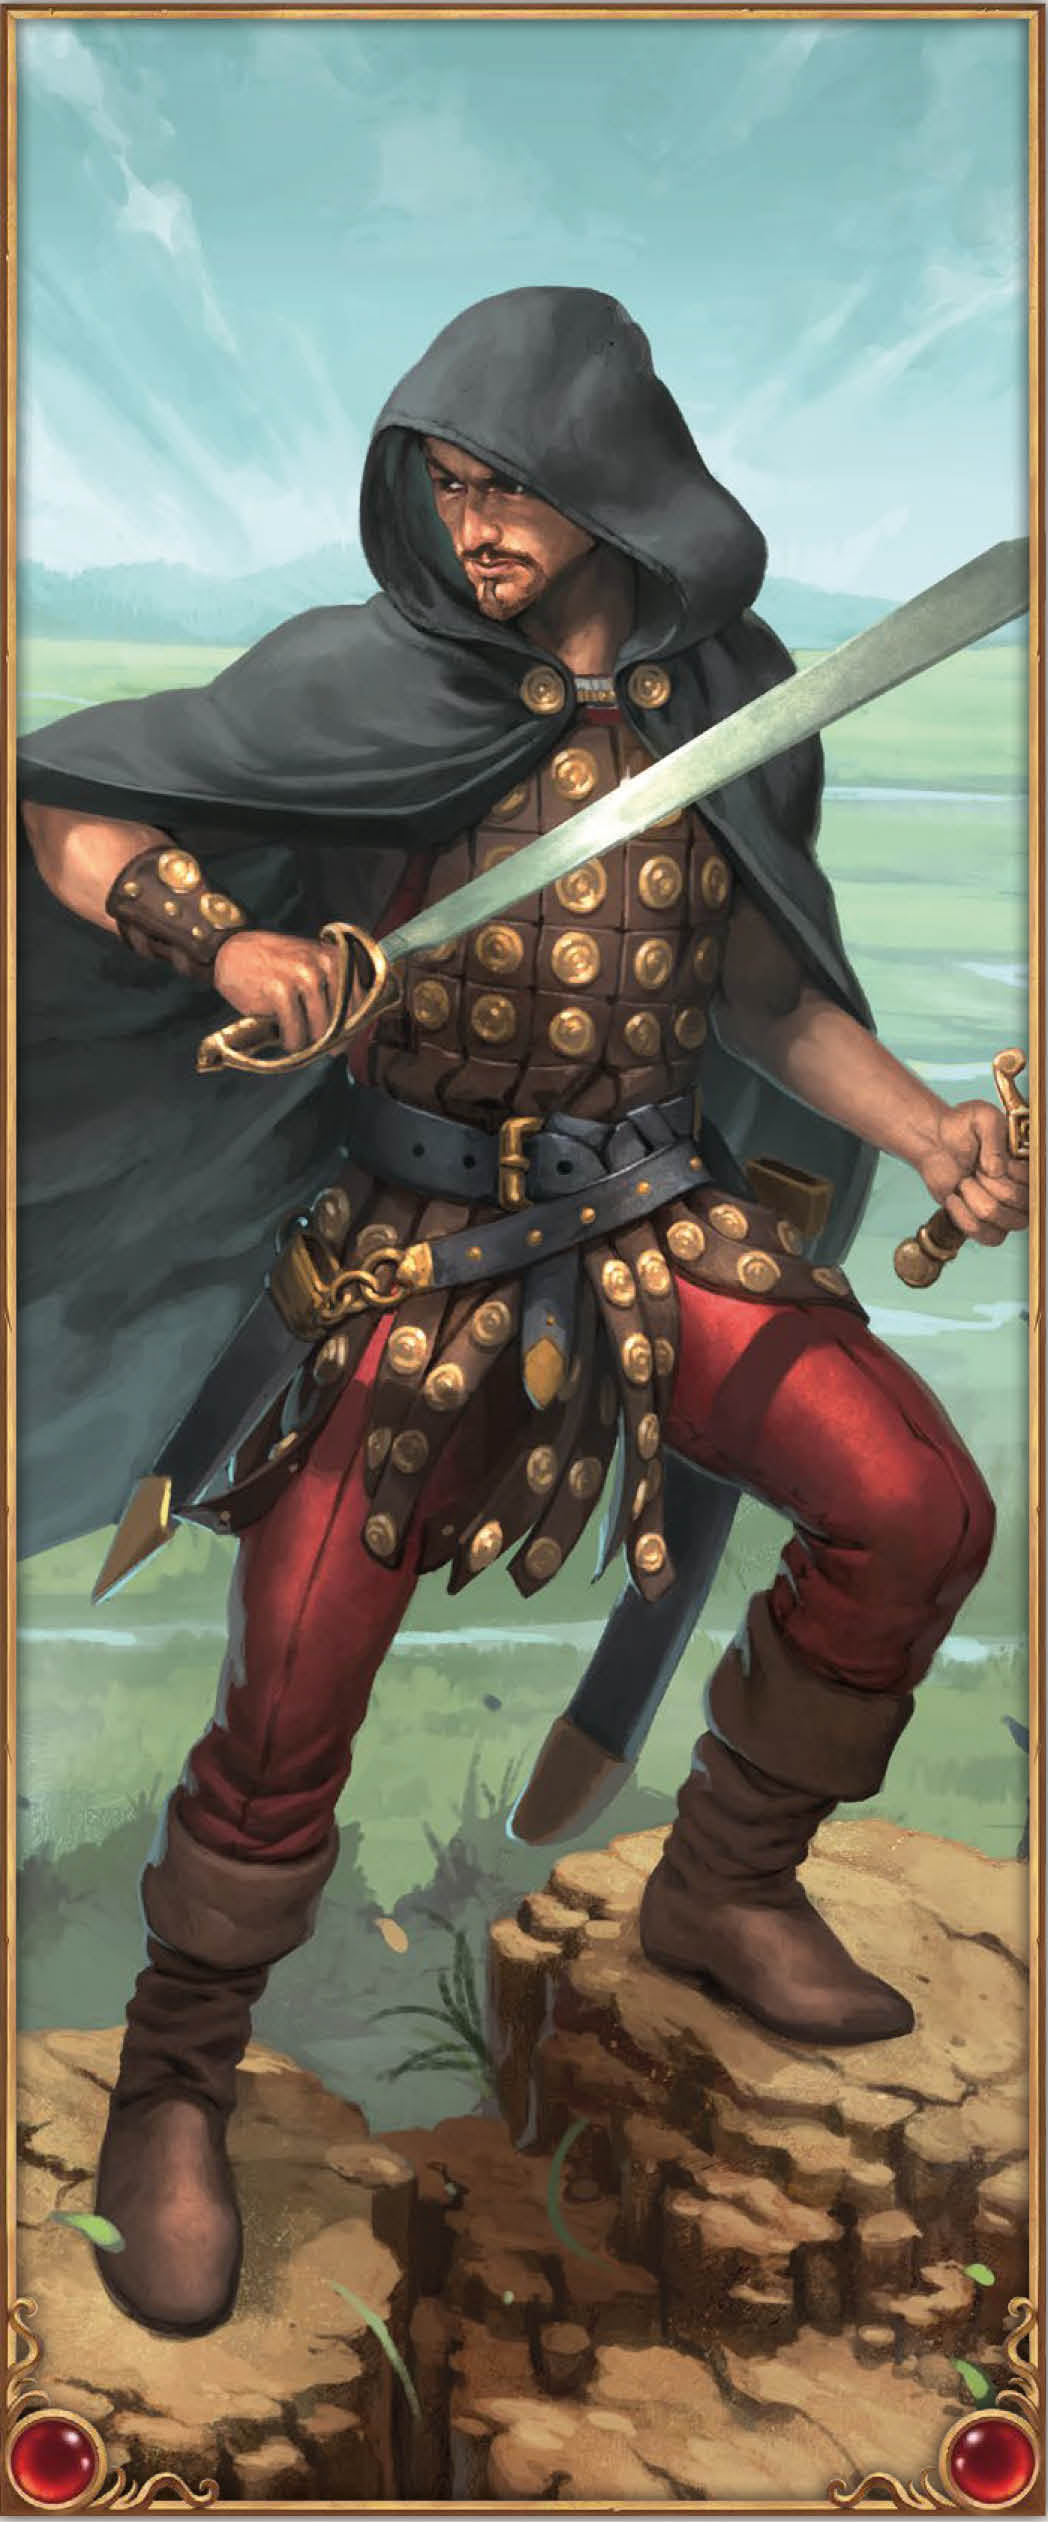
\includegraphics[width=\linewidth]{\art/rogue.jpg}

\subsection*{Combat with Neutral Units}

During Combat with Neutral Units in clash Scenarios, if a player decides to deploy their Units only on one half (left or right) of the battle Board, the player positioning the Neutral Units must do the same.

Placing Neutral Units far apart only makes the other player waste MPs, which slows the game down.
The exception to this rule is when there are three Neutral \svg{unit_ground} or \svg{unit_flying} Units to position, as all of them must go to the front line.
See examples that follow.

\begin{center}
  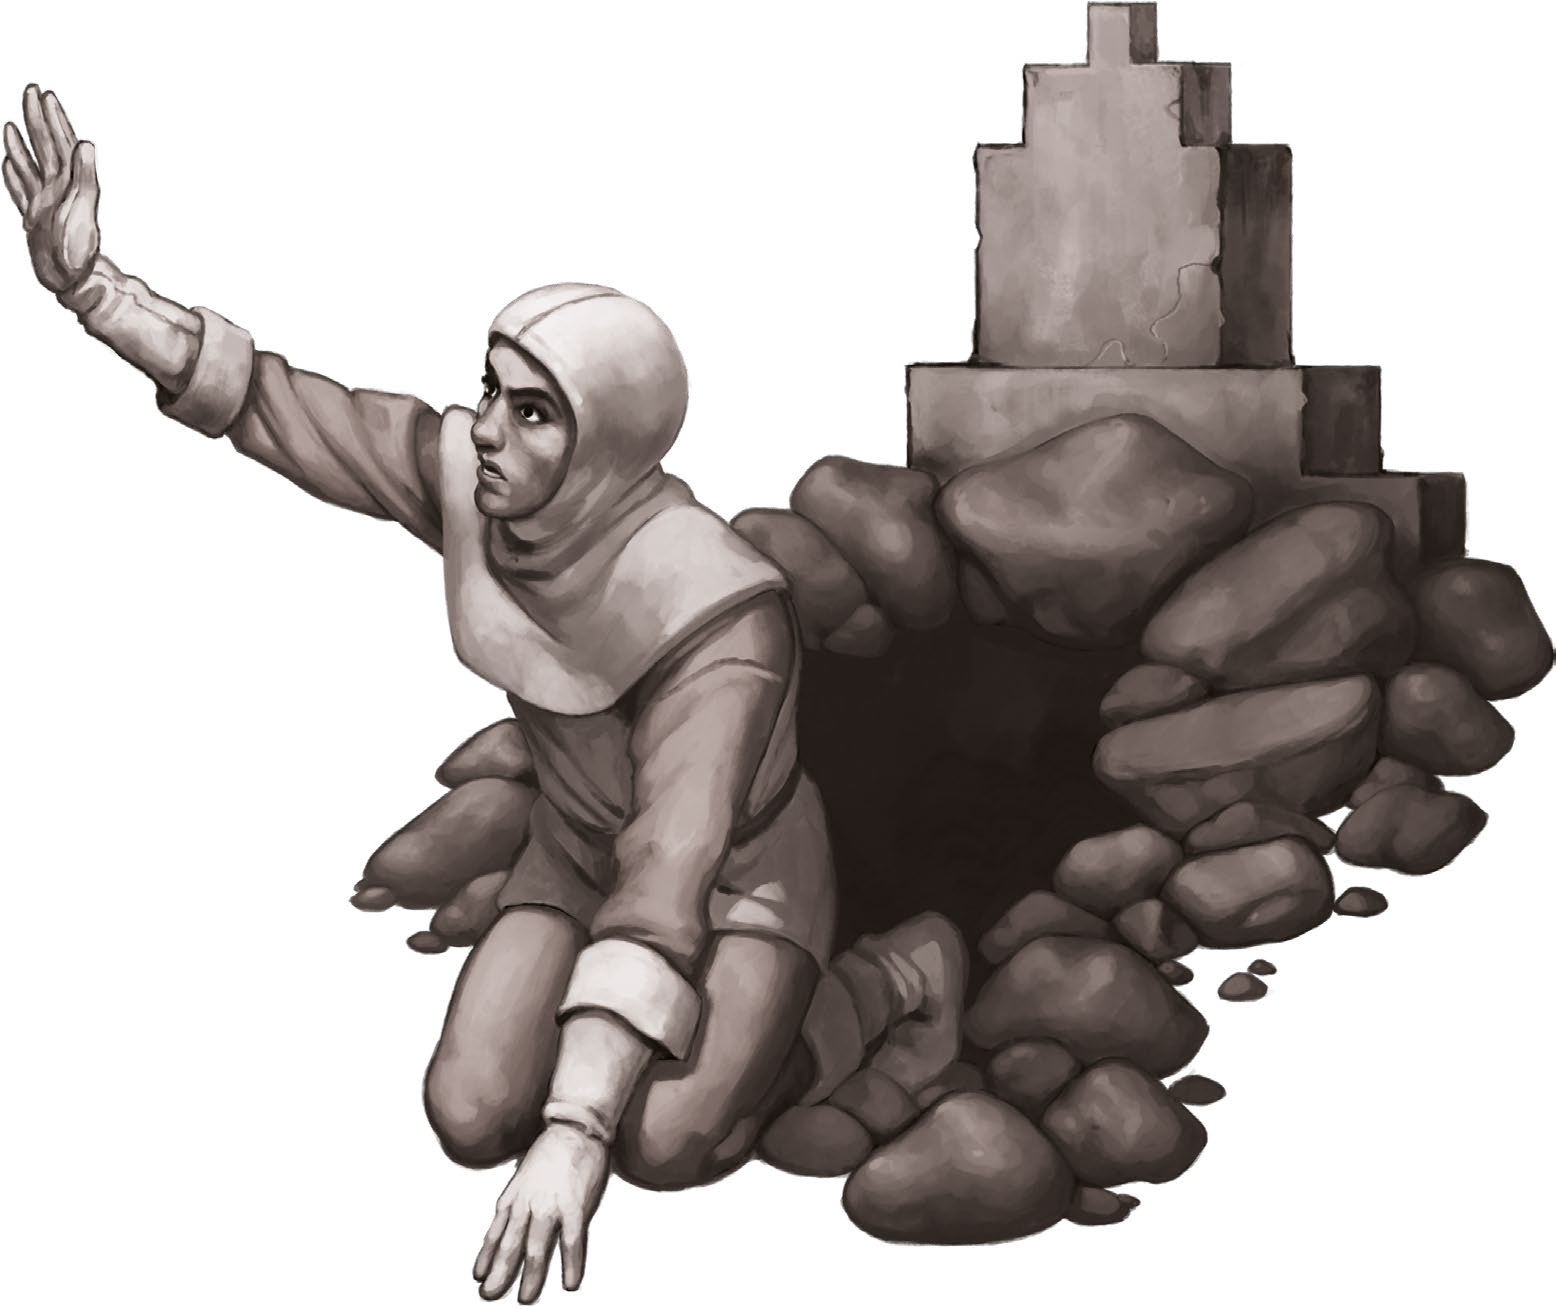
\includegraphics[width=0.65\linewidth]{\art/resurrection.png}
\end{center}

\end{multicols}

\begin{figure*}[!h]
  \mbox{}
  \hfill
  \begin{minipage}[t]{0.44\textwidth}
    \centering
    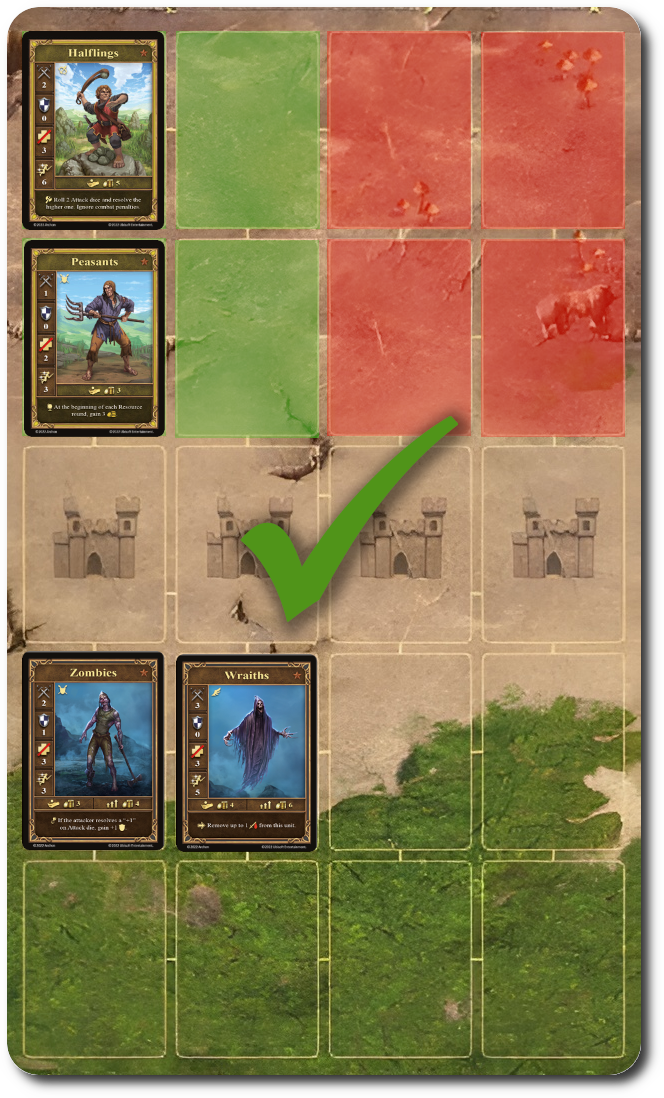
\includegraphics[width=\linewidth]{\examples/battle_good.png}
    \caption[good protected]{\textit{Neutral Units are positioned correctly.}}
  \end{minipage}
  \hfill
  \begin{minipage}[t]{0.44\textwidth}
    \centering
    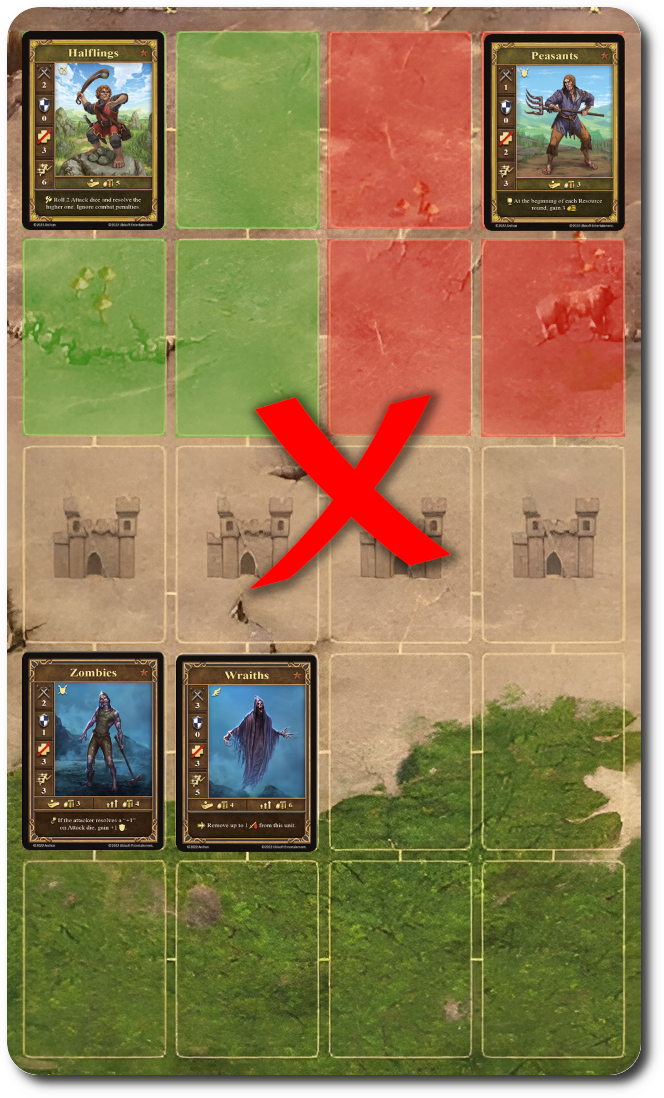
\includegraphics[width=\linewidth]{\examples/battle_bad.png}
    \caption[bad protected]{\textit{This deployment is not allowed because the Necropolis player placed their Units on the left half of the Combat Board.
      The Peasants must also start the Combat on the left side.}}
  \end{minipage}
  \hfill
  \mbox{}
\end{figure*}

\clearpage

\begin{figure*}[!h]
  \mbox{}
  \hfill
  \begin{minipage}[t]{0.44\textwidth}
    \centering
    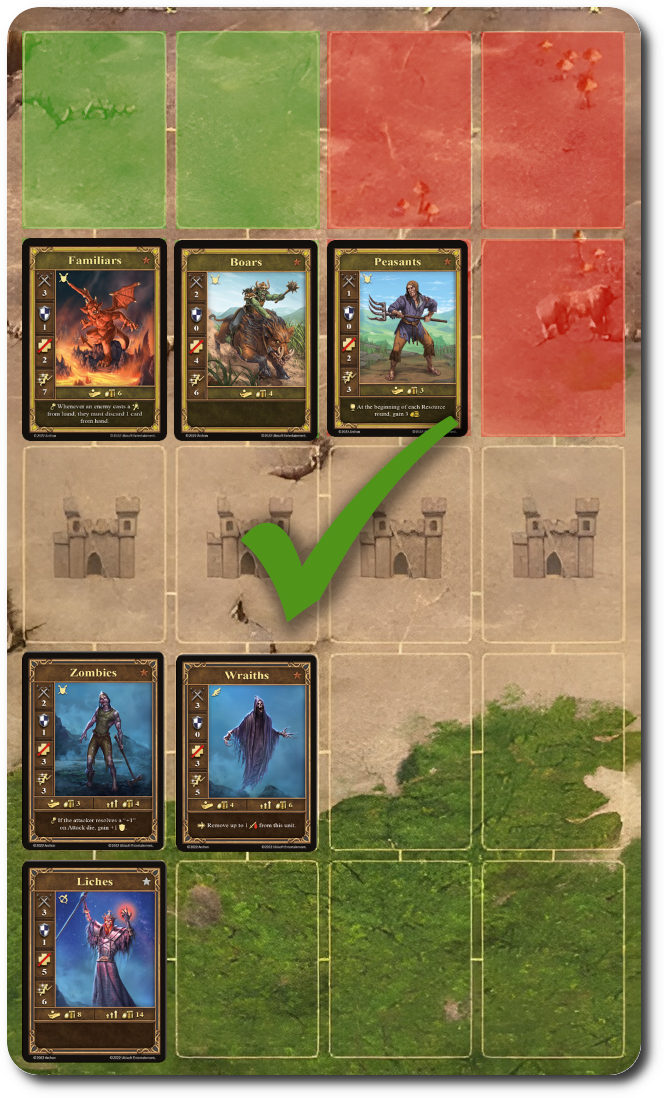
\includegraphics[width=\linewidth]{\examples/battle_exception.png}
    \caption[exception protected]{\textit{\textbf{Exception:} Three non-\svg{unit_ranged} Units must be positioned on the front line.}}
  \end{minipage}
  \hfill
  \begin{minipage}[t]{0.44\textwidth}
    \centering
    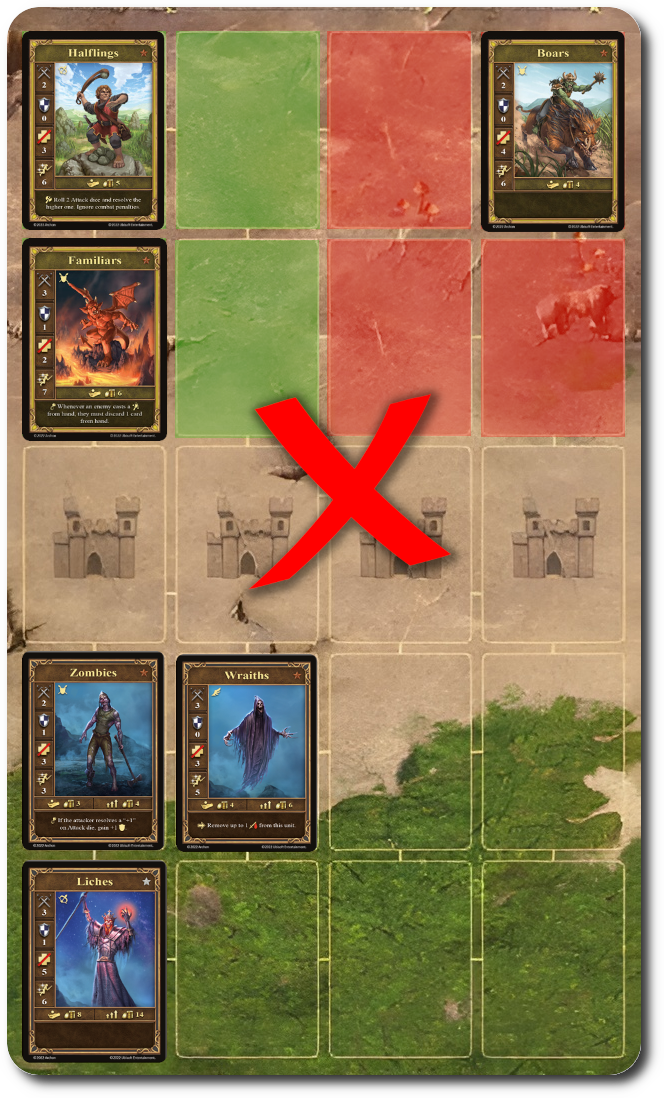
\includegraphics[width=\linewidth]{\examples/battle_ranged_bad.png}
    \caption[ranged protected]{\textit{The Boars must occupy one of the green Fields.}}
  \end{minipage}
  \hfill
  \mbox{}
\end{figure*}

\begin{multicols}{2}

\subsection*{General Recommendations}

The following are not custom rules, but rather recommendations to help you get the most out of your game:

\begin{itemize}
  \item When deciding which building to construct in your Town, especially in the early game, it is \textit{usually} best to prioritize Units over the City Hall, Citadel, Mage Guild, or other Faction-specific buildings.
  \item If you're unsure which Spell, Artifact, or Ability to choose, prioritize those that help you cycle through your Deck.
    This includes any cards that allow you to draw cards or retrieve cards from your Discard Pile.
  \item Try to avoid using your Main Hero's Movement Points for Actions that your Secondary Hero can handle, such as flipping the Map Tiles, Visiting Water Wheels, and so on.
\end{itemize}

\begin{center}
  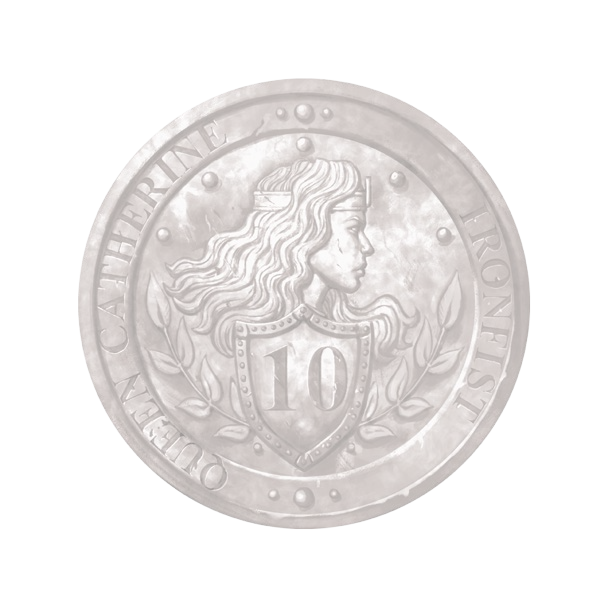
\includegraphics[width=0.7\linewidth]{\art/coin.png}
\end{center}

\end{multicols}
